\textbf{Ejemplo 7}\\
Elaborar una tabla para amortizar la suma de  3.000.000 COP en pagos trimestrales durante 15 meses con una tasa del 24\% nominal anual trimestre vencido\\ \\
%\newpage %USAR SOLO SI EL SOLUCIÓN QUEDA SOLO Y ES NECESARIO BAJARLO A LA SIGUIENTE PAGINA
\textbf{Solución.}
%La tabla ira centrada
\begin{center}
 \renewcommand{\arraystretch}{1.5}% Margenes de las celdas
 %Creación de la cuadricula de 3 columnas
 \begin{longtable}[H]{|p{0.333\linewidth}|p{0.3333\linewidth}|p{0.3333\linewidth}|}
  \hline
  \multicolumn{3}{|c|}{\cellcolor[HTML]{FFB183}\textbf{1. Declaración de variables}}             \\ \hline
  $VP= 3.000.000 COP$    & $i=6\% \hspace{1mm} ptv$                 & $R =  ? COP $               \\
  $n=5 \hspace{1mm} ptv$ & $\text{Cuota inicial}=40\% \hspace{1mm} VP$ &                         \\ \hline
  \multicolumn{3}{|c|}{\cellcolor[HTML]{FFB183}\textbf{2. Tabla de flujo de caja}}               \\ \hline
  \multicolumn{3}{|p{\columnwidth}|}{
  \begin{center}
   \begin{tabular}{|c|c|c|c|c|c|}
    \hline
    \textbf{Periodo} & \textbf{Saldo Inicial} & \textbf{Intereses} & \textbf{Abono Capital} & \textbf{Cuota} & \textbf{Saldo Final} \\ \hline
    0                &  3.000.000  COP          &  0        COP        &  0        COP            &  0        COP    &  3.000.000   COP    \\ \hline
    1                &  3.000.000  COP          &  712.189  COP        &  180.000  COP            &  532.189   COP   &  2.467.811   COP    \\ \hline
    2                &  2.467.811  COP          &  712.189  COP        &  148.069  COP            &  564.121  COP    &  1.903.690   COP    \\ \hline
    3                &  1.903.690  COP          &  712.189  COP        &  114.221  COP            &  597.968   COP   &  1.305.722   COP    \\ \hline
    4                &  1.305.722  COP          &  712.189  COP        &  78.343   COP            &  633.846  COP    &  671.877     COP    \\ \hline
    5                &  671.877    COP          &  712.189  COP        &  40.313   COP            &  671.877  COP    &  -           COP    \\ \hline
   \end{tabular}
  \end{center}
  }                                                                                              \\ \hline
  \multicolumn{3}{|c|}{\cellcolor[HTML]{FFB183}\textbf{3. Fórmulas utilizadas}}                  \\ \hline
  \multicolumn{3}{|p{\columnwidth}|}{Mediante el uso de Excel:
  \begin{itemize}
   \item PAGO: Calcula el pago de un prestamo basado en pagos y tasas de interés constantes.
  \end{itemize}
  }                                                                                              \\ \hline
  \multicolumn{3}{|c|}{\cellcolor[HTML]{FFB183}\textbf{4. Desarrollo en Excel}}                  \\ \hline
  \multicolumn{3}{|p{\columnwidth}|}{
  Se aplicará la función PAGO de la siguiente forma:

  =PAGO(0,06;5;-3000000) con referencia en la hoja de Excel usada para el ejercicio.
  }                                                                                              \\
  \multicolumn{3}{|c|}{ 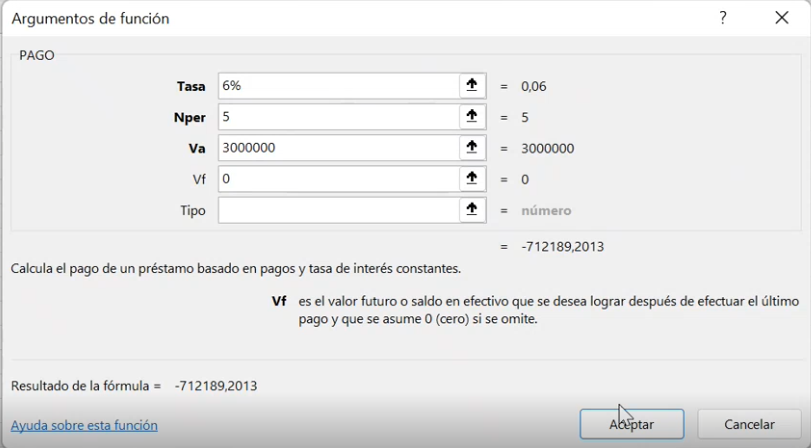
\includegraphics[trim=-5 -5 -5 -5 ,width=1\columnwidth]{7/Ejem7.PNG}}    \\
  \multicolumn{3}{|c|}{\cellcolor[HTML]{FFB183}\textbf{5. Respuesta}}                            \\ \hline
  \multicolumn{3}{|p{\columnwidth}|}{
  El pago será de 721.189 COP
  }                                                                                              \\ \hline
  \multicolumn{3}{|c|}{\cellcolor[HTML]{FFB183}\textbf{6. Grafica}}                              \\ \hline
  \multicolumn{3}{|c|}{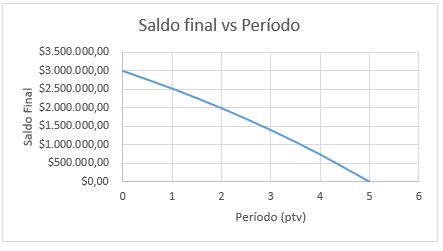
\includegraphics[trim=-5 -5 -5 -5 ,width=0.7\columnwidth]{7/grafica.png}} \\ \hline
 \end{longtable}
 %\newline \newline %USARLO SI CREES QUE ES NECESARIO
\end{center}